\section{The Dispa-SET model}

\subsection{Overview}

The Dispa-SET model \cite{dispaset} is described in the source \cite{dispaset2} as "an open-source unit commitment and optimal dispatch model focused on the balancing and flexibility problems in European grids".

More precisely, it is focused on simulating large scale power systems, with emphasis on high shares of VRES. It follows that it is used as tool for the analysis of the impacts of VRES on the power systems, thank to its ability to take into account several technical constraints of the power system.

A schematic of the Dispa-SET architecture is given in Figure \ref{dispaset-architecture}.

\begin{figure}[h]
    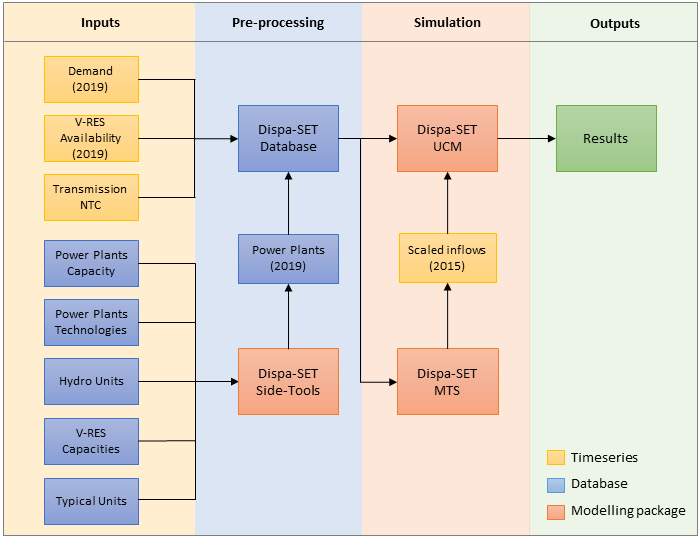
\includegraphics[width=0.9\textwidth]{dispaset-architecture.png}
    \caption{Block diagram of Dispa-SET architecture}
    \label{dispaset-architecture}
\end{figure}

Dispa-SET has several option regarding the formulation of the problem:
\begin{itemize}
    \item Linear programming (LP) optimization problem
    \item Mixed Integer Linear Programming (MILP) optimization problem.
\end{itemize}

Its interface is written in the Python programming language, and calls GAMS \cite{GAMS} as the main solver engine.

\subsection{Objective function}

The Dispa-SET model aims at minimizing the overall operating costs of the grid, that is, its objective function. These costs typically include transportation, power and heating costs required to split efficiently the demand between the available generation units.

The total system costs is splitted as follows:
\begin{itemize}
    \item \textit{Fixed cost}: fixed amount, charged if the unit is on.
    \item \textit{Variable costs}: amount that is a function of the power output the units are operating at.
    \item \textit{Start-up} and \textit{Shutdown costs}: amount charged on start and on shutdown of a unit.
    \item \textit{Ramp-up} and \textit{Ramp-down costs}: costs due to the increase or decrease in power output of a unit.
    \item \textit{Shed load costs}: costs due to necessary load sheddings.
    \item \textit{Loss of load costs}: due to generated either exceeding the demand, or not matching it .
    \item \textit{Transmission costs}: due to the use and wear of the transmission network.
    \item \textit{Spillage costs}: due to spillage in storage units.
\end{itemize}

We can formulate, Equation \ref{obj-function-sum} to represent the objective function, where $u$ refers to the index on each units, and $i$ is the time index.

\begin{captionnable}
    $Min_{TotalSystemCost}=$
    \begin{equation}
        \begin{split}
            & \sum_{u,i} (CostStartUp_{i,u} + CostShutDown_{i,u}) \:+ \\
            & \sum_{u,i} (CostRampUp_{i,u} +CostRampDown_{i,u}) \:+ \\
            & \sum_{u,i} CostFixed_{u}\cdot Comitted_{i,u} \cdot TimeStep\:+ \\
            & \sum_{u,i} CostVariable_{i,u}\cdot  Power_{i,u} \cdot TimeStep\:+ \\
            & \sum_{hu,i} CostVariable_{i,u}\cdot Heat_{i,u} \cdot TimeStep \:+ \\
            & \sum_{l,i} PriceTransmission_{i,l}\cdot Flow_{i,l} \cdot TimeStep \:+ \\  
            & \sum_{n,i} CostLoadShedding_{i,n}\cdot ShedLoad_{i,n} \cdot TimeStep \:+ \\
            & \sum_{n\_th,i} CostHeatSlack_{n\_th,i}\cdot HeatSlack_{n\_th,i} \cdot TimeStep \:+ \\ 
            & \sum_{n\_h2,i} CostH2Slack_{n\_h2,i}\cdot H2Slack_{n\_h2,i} \cdot TimeStep \:+ \\ 
            & \sum_{chp,i} CostVariable_{chp,i}\cdot CHPPowerLossFactor_{chp,i}\cdot Heat_{chp,i} \cdot TimeStep \:+  \\
            & \sum_{i,n} VOLL_{Power}·(LL_{MaxPower,i,n} +LL_{MinPower,i,n}) \cdot TimeStep \:+  \\
            & \sum_{i,n} 0.8 \cdot VOLL_{reserve}·(LL_{2U,i,n} + LL_{2D,i,n} + LL_{3D,i,n}) \cdot TimeStep \:+ \\
            & \sum_{u,i} 0.7 \cdot VOLL_{Ramp}·(LL_{RampUP,u,i} +LL_{RampDown,u,i}) \cdot TimeStep \:+\\
            & \sum_{s,i}CostOfSpillage \cdot Spillage_{s,i}
        \end{split}
        \label{obj-function-sum}
    \end{equation}
    \equationcaption{Objective function of the Dispa-SET model}
\end{captionnable}

\subsection{Supply and demand balance}

At all time and in each zone, the fundamental constraint that has to be met is the supply-demand balance in terms of energy production (supply) and consumption (demand), in the day-ahead market.

The supply sources are:
\begin{itemize}
    \item The power outputs from each units 
    \item The power outputs from storage units discharging
    \item The (eventual) net income from importation from neighbouring zones
    \item The (eventual) shed load
\end{itemize}

Whereas the demand originates from:
\begin{itemize}
    \item The load in that zone
    \item The (eventual) net exportations to neighbouring zones
    \item The power consumed by charging storage units
    \item The power consumed by P2H (power to heat) units
\end{itemize}

The Equation \ref{supply-demand-balance-equation} expresses this target equality.
\mywarning{Mieux détailler les membres de l'équation}

\begin{captionnable}
    \begin{equation}
        \begin{split}
            &\sum_{u} (Power_{u,i} \cdot Location_{u,n}) + \sum_{l} (Flow_{u,i} \cdot LineNode_{l,n})\\
            & = Demand_{DA,n,i} + Demand_{Flex,n,i} + \sum_{s} (StorageInput_{s,i} \cdot Location_{s,n}) + \\
            & \sum_{p2h}(PowerConsumption_{p2h,i} \cdot Location_{p2h,i}) - ShedLoad_{n,i} - LL_{MaxPower_{n,i}} + LL_{MinPower_{n,i}} 		
        \end{split}
        \label{supply-demand-balance-equation}
    \end{equation}
    \equationcaption{Supply-demand balance in Dispa-SET}
\end{captionnable}

\subsection{Rolling horizon}

The perfect solution would be solving the whole system, for every time step in the complete duration of the simulation in one go. But this would create a system too large to be reasonably solved.

To manage this, the simulation is split into smaller, manageable parts. The simulation is made for a smaller time frame, called the optimization period, over which the simulation can be made easily.

The start of optimization period $j$ overlaps the optimization period $j-1$, to that the simulation $j$ is the correct prolongation of the same setting fixed by the simulations up to $j-1$. The period that overlaps is called the look-ahead, in which the values of the parameters for period $j-1$ is determined during simulation $j-1$, and are used as fixed context for simulation $j$. A depiction of rolling horizon is given in Figure \ref{fig:rolling-horizon}.

\begin{figure}[h]
    \centering
    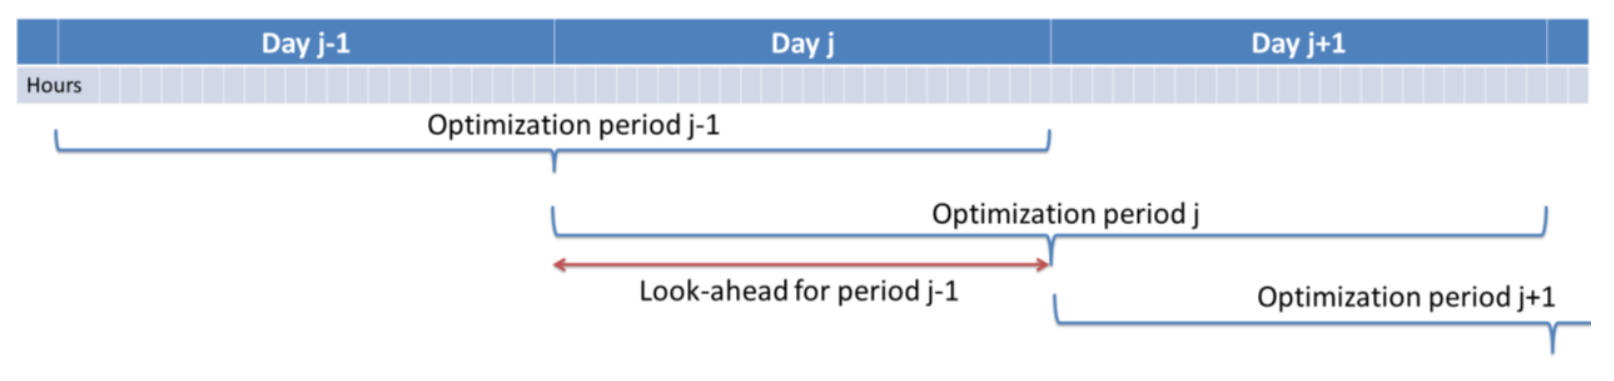
\includegraphics[width=0.9\textwidth]{resources/images/rolling_horizon.png}
    \caption{Depiction of the rolling horizon mechanism}
    \label{fig:rolling-horizon}
\end{figure}

\subsection{Mid-term scheduling}

Without further constraints, the optimization will most often leave all the storage facilities empty at the end of the simulation horizon (typically a few days). This is a consequence of the variable operational cost of discharging these storage units being smaller than the cost of running another unit, thus charging extra fixed and variable costs.

In order to tackle this issue, the Dispa-SET model has to be run in Mid-Term Scheduling (MTS) mode. In this mode, the initial and final levels of the storage units (in particular, pumped hydro storage units) are given as exogenous input to the model. These levels are enforced with additional constraints.

In this work, the MTS mode is enabled, and the exogenous inputs, for both initial and final levels, are set to half of the storage capacity.

\subsection{Dispa-SET components and representation}

Dispa-SET provides us with several predefined configurations, each of these defining the zones and their units of interest, and linking to the relevant data (e.g. times series provided as \texttt{csv} files).

In this work, the european setting is used.

\subsubsection{Zones}

Most of the EU contries are represented, for completeness they are reported in Table \ref{table:countries-eu}.

\begin{table}[h]
    \centering
	\begin{tabular}{|l l|l l|}
		\hline
		Code & Country & Code & Country \\
		\hline
		AT & Austria        & IE & Ireland \\
		BE & Belgium        & IT & Italy \\
		BG & Bulgaria       & LT & Lithuania \\
		CH & Switzerland    & LV & Latvia \\
		CZ & Czech Republic & NL & Netherlands \\
		DE & Germany        & NO & Norway \\
		DK & Denmark        & PL & Poland \\
		EE & Estonia        & PT & Portugal \\
		EL & Greece         & RO & Romania \\
		ES & Spain          & SE & Sweden \\
		FI & Finland        & SI & Slovenia \\
		FR & France         & SK & Slovakia \\
		HR & Croatia        & UK & United Kingdom \\
		HU & Hungary        & & \\
		\hline
	\end{tabular}
	\caption{Countries present in Dispa-SET EU, and their ISO Alpha 2 country codes. These are all the EU contry except for Cyprus and Malta and Luxembourg, plus Norway, Switzerland and the UK.}
	\label{table:countries-eu}
\end{table}

\subsubsection{Technologies}

Table \ref{table:technologies-eu} lists all the technologies taken into account by Dispa-SET, alongside with their main properties: 

\begin{itemize}
    \item VRES: does the technology belongs to VRES?
    \item Storage: can it store energy?
    \item Flexibility: ease of control of the unit's power output.
\end{itemize}

Due to the intermittency of their resources, and because one cannot dispatch them, VRES are considered inflexible.

However, hydroelectric units with a reservoir are have some room for flexibility, due their ability to manage their storage level.

Steam turbines, because of their dependency on the fuel used, e.g. nuclear energy would be less flexible than natural gas.

Heating and combined heat and power units are not covered, as only the electricity is of interest in this scope.

\begin{table}
    \centering
    \begin{tabular}{|l l c c c|}
        \hline
		Identifier & Description & VRES & Storage & Flexibility\\
		\hline
		COMC & Combined cycle             & No  & No  & High\\
		GTUR & Gas turbine                & No  & No  & High\\
		ICEN & Internal combustion engine & No  & No  & High\\
		STUR & Steam turbine              & No  & No  & Medium\\
		HDAM & Conventional hydro dam     & No  & Yes & Medium \\
		HROR & Hydro run-of-river         & Yes & No  & Low\\
		HPHS & Pumped hydro storage       & No  & Yes & Medium\\
		WTOF & Offshore wind turbine      & Yes & No  & Low\\
		WTON & Onshore wind turbine       & Yes & No  & Low\\
		PHOT & Solar photovoltaic         & Yes & No  & Low\\
		BATS & Stationary batteries       & No  & Yes & High\\
		\hline
    \end{tabular}
    \caption{Technologies present in Dispa-SET}
    \label{table:technologies-eu}
\end{table}


\subsubsection{Fuels}

Table \ref{table:fuels-eu} summarizes the fuel types in Dispa-SET.

It is important to highlight that technologies may not always be powered by the same fuel, for instance, the steam turbines can use most of them.

Each unit must specify its technology and fuel. Depending on the optimization problem formulation, units featuring the same (technology-fuel) pair will be grouped together and thereafter be treated as one single unit. This grouping is of crucial importance, as it will define the behaviour of the simulation when using the MILP formulation (see \ref{subsubection:milp}).

\begin{table}[h]
    \centering
	\begin{tabular}{|l l|}
		\hline
		Fuel & Description\\
		\hline
		BIO & Biofuels\\
		GAS & Gas\\
		HRD & Coal\\
		LIG & Lignite \\
		NUC & Nuclear energy\\
		OIL & Petroleum\\
		PEA & Peat Moss\\
		GEO & Geothermal steam \\
		SUN & Solar energy\\
		WAT & Hydro energy\\
		WIN & Wind energy\\
		WST & Energy from waste\\
		OTH & Other fuels and energy carriers\\
		\hline
	\end{tabular}
	\caption{Fuel types in Dispa-SET}
	\label{table:fuels-eu}
\end{table}

A major consideration for the optimization problem is the fuel prices, which are listed in Table \ref{table:fuel-prices}.

A key feature is the relationship between the price of coal and the price of gas: depending on which one is the cheaper, the optimal behaviour change dramatically. Obviously, the cheapest one will always be preferred over the other when choice arise. 

\begin{table}[h]
    \centering
	\begin{tabular}{|l c|}
		\hline
		& Price \\
		\hline
		Nuclear    & 3 \\
		Black coal & 20 \\
		Gas        & 45 \\
		Fuel-Oil   & 65\\
		Biomass    & 10.08\\
		Lignite    & 7.23\\
		Peat       & 9.36 \\
		\hline
	\end{tabular}
	\caption{Fuel prices considered, in €/MWh}
	\label{table:fuel-prices}
\end{table}

\subsubsection{Other prices}

Some other price values are relevant, such as the price of the load shedding per MWh. These are presented in Table \ref{table:other-prices}.

\begin{table}[h]
    \centering
	\begin{tabular}{|l c|}
		\hline
		What & Price \\
		\hline
		CO2                & 25 \\
		Unserved Heat      & 84.21\\
		Load Shedding Cost & 1000\\
		Transmission       & 0\\
		Unserved H2        & 75\\
		Curtailment Cost   & 20 \\
		\hline
	\end{tabular}
	\caption{Other relevant prices, in €/MWh}
	\label{table:other-prices}
\end{table}

\mywarning{prix du CO2 en euro/MWh}

These values define the significance of each problem relatively to each other, hence what option is the least costly. For instance, the shedding cost could be so low compared to the carbon emissions that it is preferable not to run any coal unit to produce 1MW than to shed 1MW. This example is extreme, but outlines the fact that these prices impact the simulation outcome via their use in the objective function.

\subsubsection{Power plants}

As a dispatch model, Dispa-SET oviously has to model the units it dispatches, namley the power plants that are present in each of the modelled zones.

For performance reasons, some of the units initially described are merged into clustered units at the pre-processing step. Thus, the amount of variable in the simulation is reduced, while the accuracy is not significantly impacted \cite{dispaset}.

Dispa-SET disposes of utilities to do so, but also needs to craft the new, aggregated units properties table. These are defined by the set of feilds that are shown in Table \ref{table:plant-db}.

\begin{table}[h]
    \centering
    \begin{tabular}{|l l l|}
        \hline
        Field           & Description                       & Type                    \\ \hline
        Unit            & Unit name                         & string                  \\
        PowerCapacity   & Maximum power output              & value in MW             \\
        Nunits          & Number of initial units clustered & integer                 \\
        Zones           & The unit's zone                   & string                  \\
        Fuel            & The fuel used                     & string                  \\
        Efficiency      & The unit's efficiency             & real in [0,1]           \\
        MinEfficiency   & Efficiency at minimum load        & real in [0,1]           \\
        MinUpTime       & Minimum up time                   & value in hours          \\
        MinDownTime     & Minimum down time                 & value in hours          \\
        RampUpRate      & Ramp up rate                      & value in minute$^{-1}$  \\
        RampDownRate    & Ramp down rate                    & value in minute$^{-1}$  \\
        RampingCost     & Cost of ramping up or down        & value in €/hour         \\
        StartUpCost\_pu & Start up cost per clustered unit  & value in €              \\
        NoLoadCost\_pu  & Cost of having no load on a unit  & value in €/hour         \\
        PartLoadMin     & Ratio of the minimum nominal capacity & real in [0,1]       \\
        StartUpTime     & Time to start up the plant        & value in hour           \\
        CO2Intensity    & Amount of CO$_2$ emitted per MW   & value in €/MW           \\ \hline
    \end{tabular}
    \caption{The table fields used to describe a optionnally aggregated power plant unit}
    \label{table:plant-db}
\end{table}

For the storage units, one needs some more parameters, given in Table \ref{table:plant-storage-db}. These feilds will remain blank for the other unit types.

\begin{table}[h]
    \centering
    \begin{tabular}{|l l l|}
        \hline
        Field                 & Description                       & Type          \\ \hline
        STOCapacity           & The total energy storage capacity & value in MWh  \\
        STOSelfDischarge      & The discharge rate (w.r.t. to the total) & value in day$^{-1}$ \\
        STOMaxChargingPower   & Maximum energy inflow             & value in MW   \\
        STOChargingEfficiency & The unit's charging efficiency    & real in [0,1] \\ \hline
    \end{tabular}
    \caption{Fields describing the storage capabilities of the units}
    \label{table:plant-storage-db}
\end{table}


Their discharge efficiency will be assigned to the common Efficiency field, and the PowerCapacity will be assigned the power output on discharge.

For batteries units, the RampUpRate and RampDownRate fields are set to 1, while the others but efficiency are set to 0. 

The crucial capability of storage units is their storage volume. In previous work in this context, the number of hours a unit can run at maximum output capacity is fixed as 4 hours, thus implicitly fixing a storage capacity given a power output.

This choice is arbitrary and leads to a simplification of the reality, where one could find huge differences in this ratio. To remove this, an option is added in Dispa-SET's adjusting function, to be able to filter the adjustments by range, making it now able to discriminate the units based on the storage capacity over maximum output power ratio, enabling its use to adjust storage units with different "longevity" separately.

However in reality, most of the difference is between the pumped hydro storage, that can typically output their maximum power for a longer time, and the other storage technologies, such as batteries.

At the end, this differenciation is not done, as it would also require the inputs of the surrogate model to be changed, to take into account the share of "high-longevity" storage units with respect to the "low-lengevity" ones.

\subsubsection{Notes on the other inputs}

We can make a few miscellaneous remarks about Dispa-SET input data.

\begin{itemize}
    \item The electricity demand is a time series from year 2019, per zone. It is assumed to be independent of the price.
    \item The net transfer capacities (NTC) between the different zones are given as inputs as hourly times series over a year. Then the maximum is picked and it is assumed that it remains constant over the year.
    \item The availability factors (AF) for renewable energy sources, defined as the ratio of the nominal power that is possible to output hourly. It is given as an hourly time series (adimentional).
    
    This variable energy generation is either curtailed or sent to the grid.

    Non-renewable technologies have their AF set to 1.

    In this work, AF denotes the hourly capacity factor, and CF (Capacity Factor) refers to the annual value. Hence, the capacity factor is the yearly average of the availability factor. 
\end{itemize}

\subsection{Problem formulations}

Dispa-SET features several, different formulations, that have a significant impact on the realism and accuracy of the output. These formulation differ in the way the simulation is created and the constraints defined.

\subsubsection{Linear programming}

In the LP formulation, every variable is considered to be continuous, and can take values down to zero.

In particular, this constraint applies to the power output of each unit, that is, the ratio of the actual power the unit is operating over its maximum capacity. Therefore, as a unit cannot produce more than its maximum capacity, this value must lie in the $[0, 1]$ interval at every hour of the simulation.

This constrain causes a significant issue, in the extent that each unit cannot specify a minimal level of operation, e.g. $0.5$. This leads to unrealistic situations being considered valid, for example a nuclear unit operating at 10\% of its maximal power.

\subsubsection{Binary formulation}

To mitigate the issue encountered with the LP formulation, it is extended by adding a boolean variable to each unit, which determines wether or not the corresponding unit is started or not. That way, the minimum operating value can be enforced.

This strategy, however acheiving the better accuracy targetted, is unfortunately often intractable for realistic settings, because the large number of binary variables, yields an exploding number of $2^N$ options to be examinated.

\subsubsection{Mixed integer linear programming \label{subsubsection:milp}}

The MILP formulation is created to leverage the computational cost of the simulation while keeping a good level of accuracy. The main idea is to group the units that share similar properties together, and only keep track of the number of units in each group that are currently running.

This permits the number of options to explore reasonnable, without hurting the precision of the output.

In this work, the MILP formulation is chosen due to its better efficiency-to-computational-cost trade-off.